\chapter{System reduction for displacement solvers}

\modinfo{Module name}{\Idx{RigidBodyReduction}}
\modinfo{Module subroutines}{RigidBody}

\begin{versiona}
\modinfo{Module authors}{Antti Pursula}
\modinfo{Document authors}{Antti Pursula}
\modinfo{Document edited}{August 27th 2003}


\section{Introduction}

\index{reduced order model} This module is used to reduce and simplify
the computation of a displacement solver when the problem includes
rigid blocks. In such a case, it is often difficult for iterative
solvers to find a solution for the full system, and direct solvers
become obsolite when the system is large enough. The convergence and
also the speed of the solution can be substantially improved when the
degrees of freedom corresponding to the nodes belonging in the rigid
blocks are reduced onto the 6~DOFs (3~in~2D) of the corresponding
rigid body. In the module, the reduction is achieved via a
\Idx{projection matrix}.

Additionally, the routine automatically eliminates the degrees of
freedom corresponding to the Dirichlet boundary conditions. It is also
possible to request the elastic regions to be extended into the rigid
blocks. There is also possibility to reorder the reduced matrix
elements to decrease its bandwidth. 


\section{Theory}

The module starts with normally constructed matrix equation for the
unknown displacements $x$, $Ax=b$. Let us assume that the nodes are
ordered in such a way that the first $n$ elements of the vectors
correspond to the elastic parts of the structure and the remaining $m$
elements correspond to the rigid parts of the structure. The goal is
to reduce the $(n+m)\times (n+m)$ matrix $A$ to a $(n+\alpha k)\times
(n+\alpha k)$ matrix $B$, where $k$ is~3 for 2D and~6 for 3D problems
and $\alpha$ is the number of rigid blocks present. Reductions are
made also for the vectors so that finally the matrix equation reads
$Bu = f$.

The relation between the unknowns is 
\begin{equation}
x = Pu,
\end{equation}
where the projection matrix $P$ ties the nodes in the rigid bodies to
the same displacements in coordinate directions and the same rotations
about the coordinate axis. The rotations are defined with a coordinate
system whose origin is at the center of each rigid body.  For the right
hand sides we can write
\begin{equation}
f = Qb,
\end{equation}
where the matrix $Q$ sums the forces and torques present at the nodes
in rigid bodies for a resultant force and torque of the center point
of the corresponding rigid body. In both mappings, the rotations are
linearized so the module is valid only for cases where the rotations
are small.

Using these definitions, we have
\begin{equation}
Ax=APu=b
\end{equation}
and
\begin{equation}
Bu=f=Qb.
\end{equation}
Combining the equations gives $Bu=QAPu$ and thus
\begin{equation}
B = QAP.
\end{equation}
With a suitable order of the rotations one can write 
\begin{equation}
Q=P^T \equiv C,
\end{equation}
and
\begin{equation}
B = CAC^T.
\end{equation}
The matrix $C$ has a identity matrix block of size $n\times n$ which
keeps the elastic nodes intact, and a projection block of size
$\alpha k\times m$. 

The reduced order solution $u$ is transformed back to the original
nodes by the same mapping
\begin{equation}
x=C^T u.
\end{equation}


\section{Applicable cases and limitations}

The module works for
\begin{itemize}
\item Linear steady-state problems
\item Linear transient problems
\item Eigen analysis
\item Quadratic eigenproblems
\end{itemize}
%
There are following limitations:
\begin{itemize}
\item Rigid blocks should not have common nodes (there should be
elastic nodes in between rigid blocks)
\item If a Dirichlet bc is given on a node of a rigid block then the
entire rigid block is assumed to be fixed in all directions
\end{itemize}



\section{Keywords}
\end{versiona}

\sifbegin
\sifitemnt{Body}{body id}
\sifbegin
  \sifitem{Rigid Body}{Logical}
Value {\tt True} defines the rigid body.
\sifend
\sifitem{Solver}{solver id}
The module does not need a separate solver but
a call in the stress analysis,
or the elasticity solver in the linear mode. 
\sifbegin
\sifitemnt{Equation}{String Stress Analysis}
\sifitemnt{Variable}{String Displacement}
\sifitem{Variable DOFs}{Integer}
It is important to give the DOFs right, either 2 or 3 depending on
the dimension.
\sifitem{Before Linsolve}{File "RigidBodyReduction"\ "RigidBody"}
The model order reduction is performed after the matrix has been assembled
but before the matrix equation has been solver. The matrix equation is 
modified to a smaller equation and the new equation is solved within the subroutine.
\sifitem{Eigen Analysis}{Logical}
It is possible to use the model order reduction with modal analysis, as
well as with static and transient cases.
\sifitem{Eigen System Values}{Integer}
The number of eigen values to be computed.
\sifitemnt{Eigen System Damped}{Logical}
\sifitem{Eigen System Use Identity}{Logical [True]}
The reduction is possible also with quadratic (damped) eigenproblems.
\sifitem{Optimize Matrix Structure}{Logical}
If true, the matrix structure is optimized. This feature is recommended 
since the reduced matrix has often very scattered structure. The
optimization is performed with the Cutholl-McKee algorithm.
\sifitem{Reverse Ordering}{Logical}
This flag can be used to reverse the matrix ordering if the matrix
structure is optimized, resulting in reverse Cuthill-McKee ordering.
\sifitem{Extend Elastic Region}{Logical}
If true, the elastic regions of the geometry are extended into the rigid 
block. This feature allows taking into account the bending in the joints 
between elastic and rigid parts.
\sifitem{Extend Elastic Layers}{Integer}
Defines the number of element layers that the elastic regions are extended.
\sifitem{Output Node Types}{Logical}
Writes in the ElmerPost output file a variable describing the status of 
each node in the geometry. The variable has value 0 for elastic nodes,
-1 for rigid blocks that are fixed due to a Dirichlet boundary condition,
and a positive integer for separate rigid blocks. The variable may be 
used to check that the reduction is performed on the right blocks, and to
check how many layers the elastic regions should be extended, for example.
\sifitem{Additional Info}{Logical}
If true, additional information is written about the performed tasks
during the simulation. 
\sifend
\sifend


\begin{versiona}
\section{Examples}

\begin{figure}[tbhp]
  \vspace{-25mm}
  \centerline{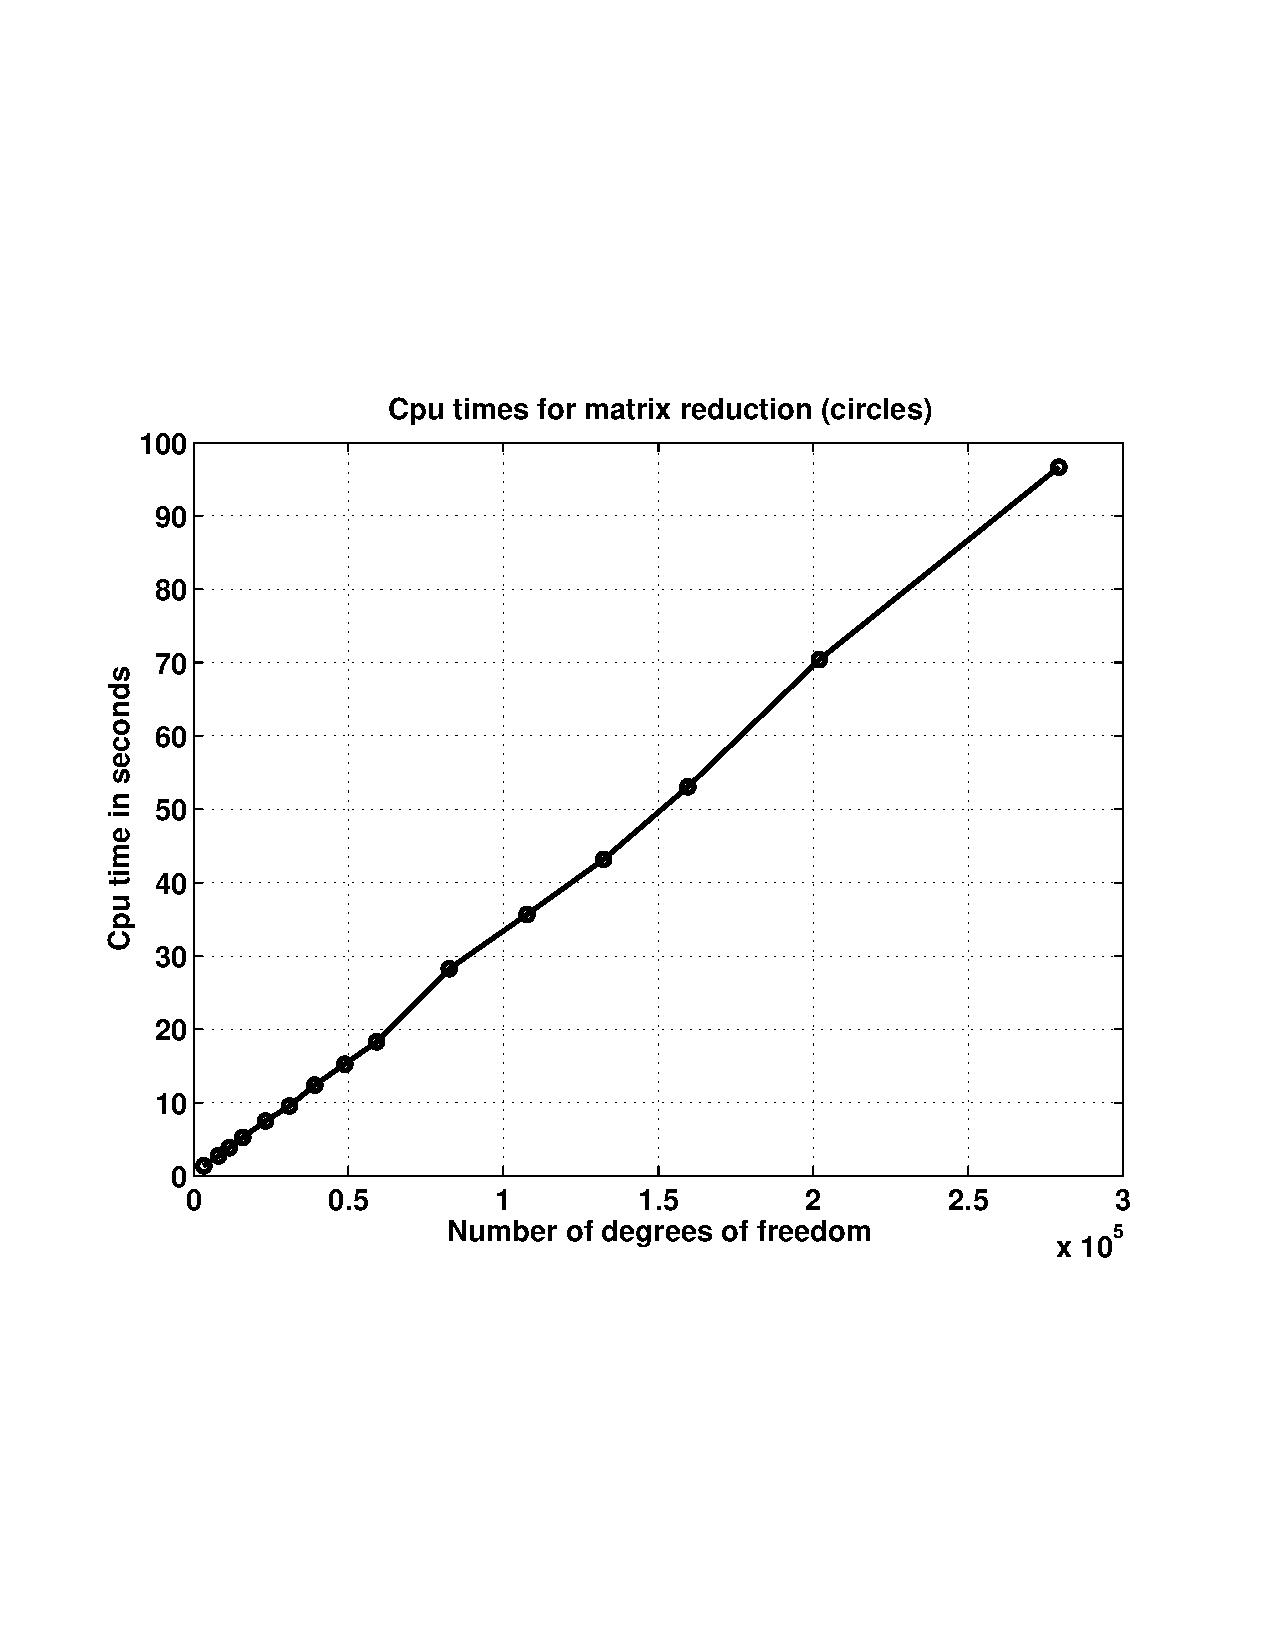
\includegraphics[width=0.6\textwidth]{reduction_cpu.pdf}}
  \vspace{-25mm}
  \caption{The cpu time required for the matrix reduction operations
  depends linearly on the degrees of freedom in the system.}
\end{figure}

%\begin{figure}[tbhp]
%  \centerline{\includegraphics[width=0.5\textwidth]{modes.ps}}
%  \caption{Two eigenmodes (1st and 5th) of a supported structure
%  calculated using matrix reduction.}
%\end{figure}

\end{versiona}
